
\documentclass{ieeeaccess}

\usepackage{cite}
\usepackage{amsmath,amssymb,amsfonts}
\usepackage{graphicx}
\usepackage{textcomp}
\usepackage{xcolor}
\usepackage{booktabs}
\usepackage{multirow}
\usepackage{url}
\usepackage{hyperref}

\newcommand{\orcidlink}[1]{\href{https://orcid.org/#1}{\raisebox{-0.25ex}{
\includegraphics[height=1.7ex]{figures/orcid.pdf}}}}
\usepackage{etoolbox}
\NewSpotColorSpace{PANTONE}
\AddSpotColor{PANTONE} {PANTONE3015C} {PANTONE\SpotSpace 3015\SpotSpace C} {1 0.3 0 0.2}
\SetPageColorSpace{PANTONE}
\usepackage{bm}
\makeatletter
\AtBeginDocument{\DeclareMathVersion{bold}
\SetSymbolFont{operators}{bold}{T1}{times}{b}{n}
\SetSymbolFont{NewLetters}{bold}{T1}{times}{b}{it}
\SetMathAlphabet{\mathrm}{bold}{T1}{times}{b}{n}
\SetMathAlphabet{\mathit}{bold}{T1}{times}{b}{it}
\SetMathAlphabet{\mathbf}{bold}{T1}{times}{b}{n}
\SetMathAlphabet{\mathtt}{bold}{OT1}{pcr}{b}{n}
\SetSymbolFont{symbols}{bold}{OMS}{cmsy}{b}{n}
\renewcommand\boldmath{\@nomath\boldmath\mathversion{bold}}}
\makeatother

\def\BibTeX{{\rm B\kern-.05em{\sc i\kern-.025em b}\kern-.08em
    T\kern-.1667em\lower.7ex\hbox{E}\kern-.125emX}}

\history{Date of publication xxxx 00, 0000, date of current version xxxx 00, 0000.}
\doi{10.1109/ACCESS.2024.0429000}
\headname{Research Article}

\begin{document}

\title{From Hand-Drawn Schematics to Structural Circuit Netlists: A Deterministic Pipeline with Endpoint-Graph Wire Joining and a Human-Verified Connectivity Benchmark}

% ORCID: add each author's ORCID before submission, e.g.
%   \uppercase{Bosco Chanam}\authorrefmark{1}~\orcidlink{0000-0000-0000-0000}
\author{\uppercase{Bosco Chanam}\authorrefmark{1}~\orcidlink{0009-0009-2527-0967},
\uppercase{Chris Dcosta}\authorrefmark{1}~\orcidlink{0009-0007-7295-0573},
\uppercase{Pranavesh Kumar Talupuri}\authorrefmark{2}~\orcidlink{0009-0005-8974-2012},
\uppercase{Shwetambari Chiwhane}\authorrefmark{1}~\orcidlink{0000-0002-3534-9654},
\uppercase{Ashay Kumar Singh}\authorrefmark{1}~\orcidlink{0009-0004-9105-7383},
and \uppercase{Arghadeep Das}\authorrefmark{1}~\orcidlink{0009-0000-9207-7694}}
\address[1]{Symbiosis Institute of Technology, Pune 412115, India (e-mail: boscochanam@gmail.com; chrisdcosta777@gmail.com; shwetambari.chiwhane@sitpune.edu.in; ashay.sit@gmail.com; arghadeep.das.work@gmail.com)}
\address[2]{Department of Computer Science, University of Southern California, Los Angeles, CA 90089 USA (e-mail: talupuri@usc.edu)}
\tfootnote{This work received no external funding.}

\markboth
{Chanam \headeretal: From Hand-Drawn Schematics to Structural Circuit Netlists}
{Chanam \headeretal: From Hand-Drawn Schematics to Structural Circuit Netlists}

\corresp{Corresponding author: Bosco Chanam (e-mail: boscochanam@gmail.com).}

\begin{abstract}
We present a deterministic pipeline for structural circuit-netlist recovery using an occlusion-first wire extractor, an endpoint graph, and degree-budget completion. The output represents inferred pin-to-node assignments; our component-pair metric does not certify pin identities, exact net partitions, absence of shorts, or simulation equivalence. Illustrative SPICE export requires externally specified values and device models; simulation equivalence on real scans is not validated. We provide a synthetic perturbation protocol and a human-verified connectivity benchmark of 31 CGHD-1152 images. With annotated component boxes and detected wires, the join achieves component-pair micro-F1 0.890 (macro-F1 0.901), compared with 0.805 for Hough plus proximity and 0.624 for connected-component tracing on the same detected wires. The wire extractor achieves F1 0.976 on 134 images with annotated component boxes under the historical benchmark configuration. Under the same component priors on the 31-image benchmark, a vision-language model reaches micro-F1 0.923; the paired difference is $+0.033$, with 95\% confidence interval $[-0.009,+0.078]$. Inclusion of zero does not establish equivalence or comparative cost superiority. These results provide within-corpus evidence, not validation of autonomous reconstruction or unseen-style generalization.
\end{abstract}

\begin{keywords}
circuit digitization, connectivity benchmark, graph-based connectivity, hand-drawn circuits, image-to-netlist, netlist extraction, schematic recognition, SPICE, wire extraction, wire joining
\end{keywords}

\titlepgskip=-21pt

\maketitle

\begin{figure*}[t]
\centering
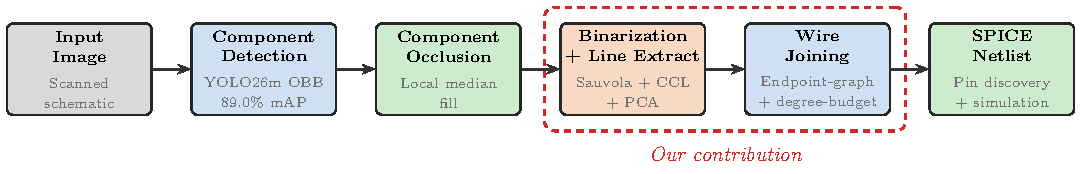
\includegraphics[width=\textwidth]{figures/pipeline_overview.pdf}
\caption{Pipeline for structural circuit-netlist recovery. The highlighted stages extract wire endpoints and infer connectivity. The net-level experiments use annotated component boxes to isolate joining; they do not establish an end-to-end error hierarchy or validate illustrative SPICE export.}
\label{fig:pipeline}
\end{figure*}

\begin{figure*}[t]
\centering
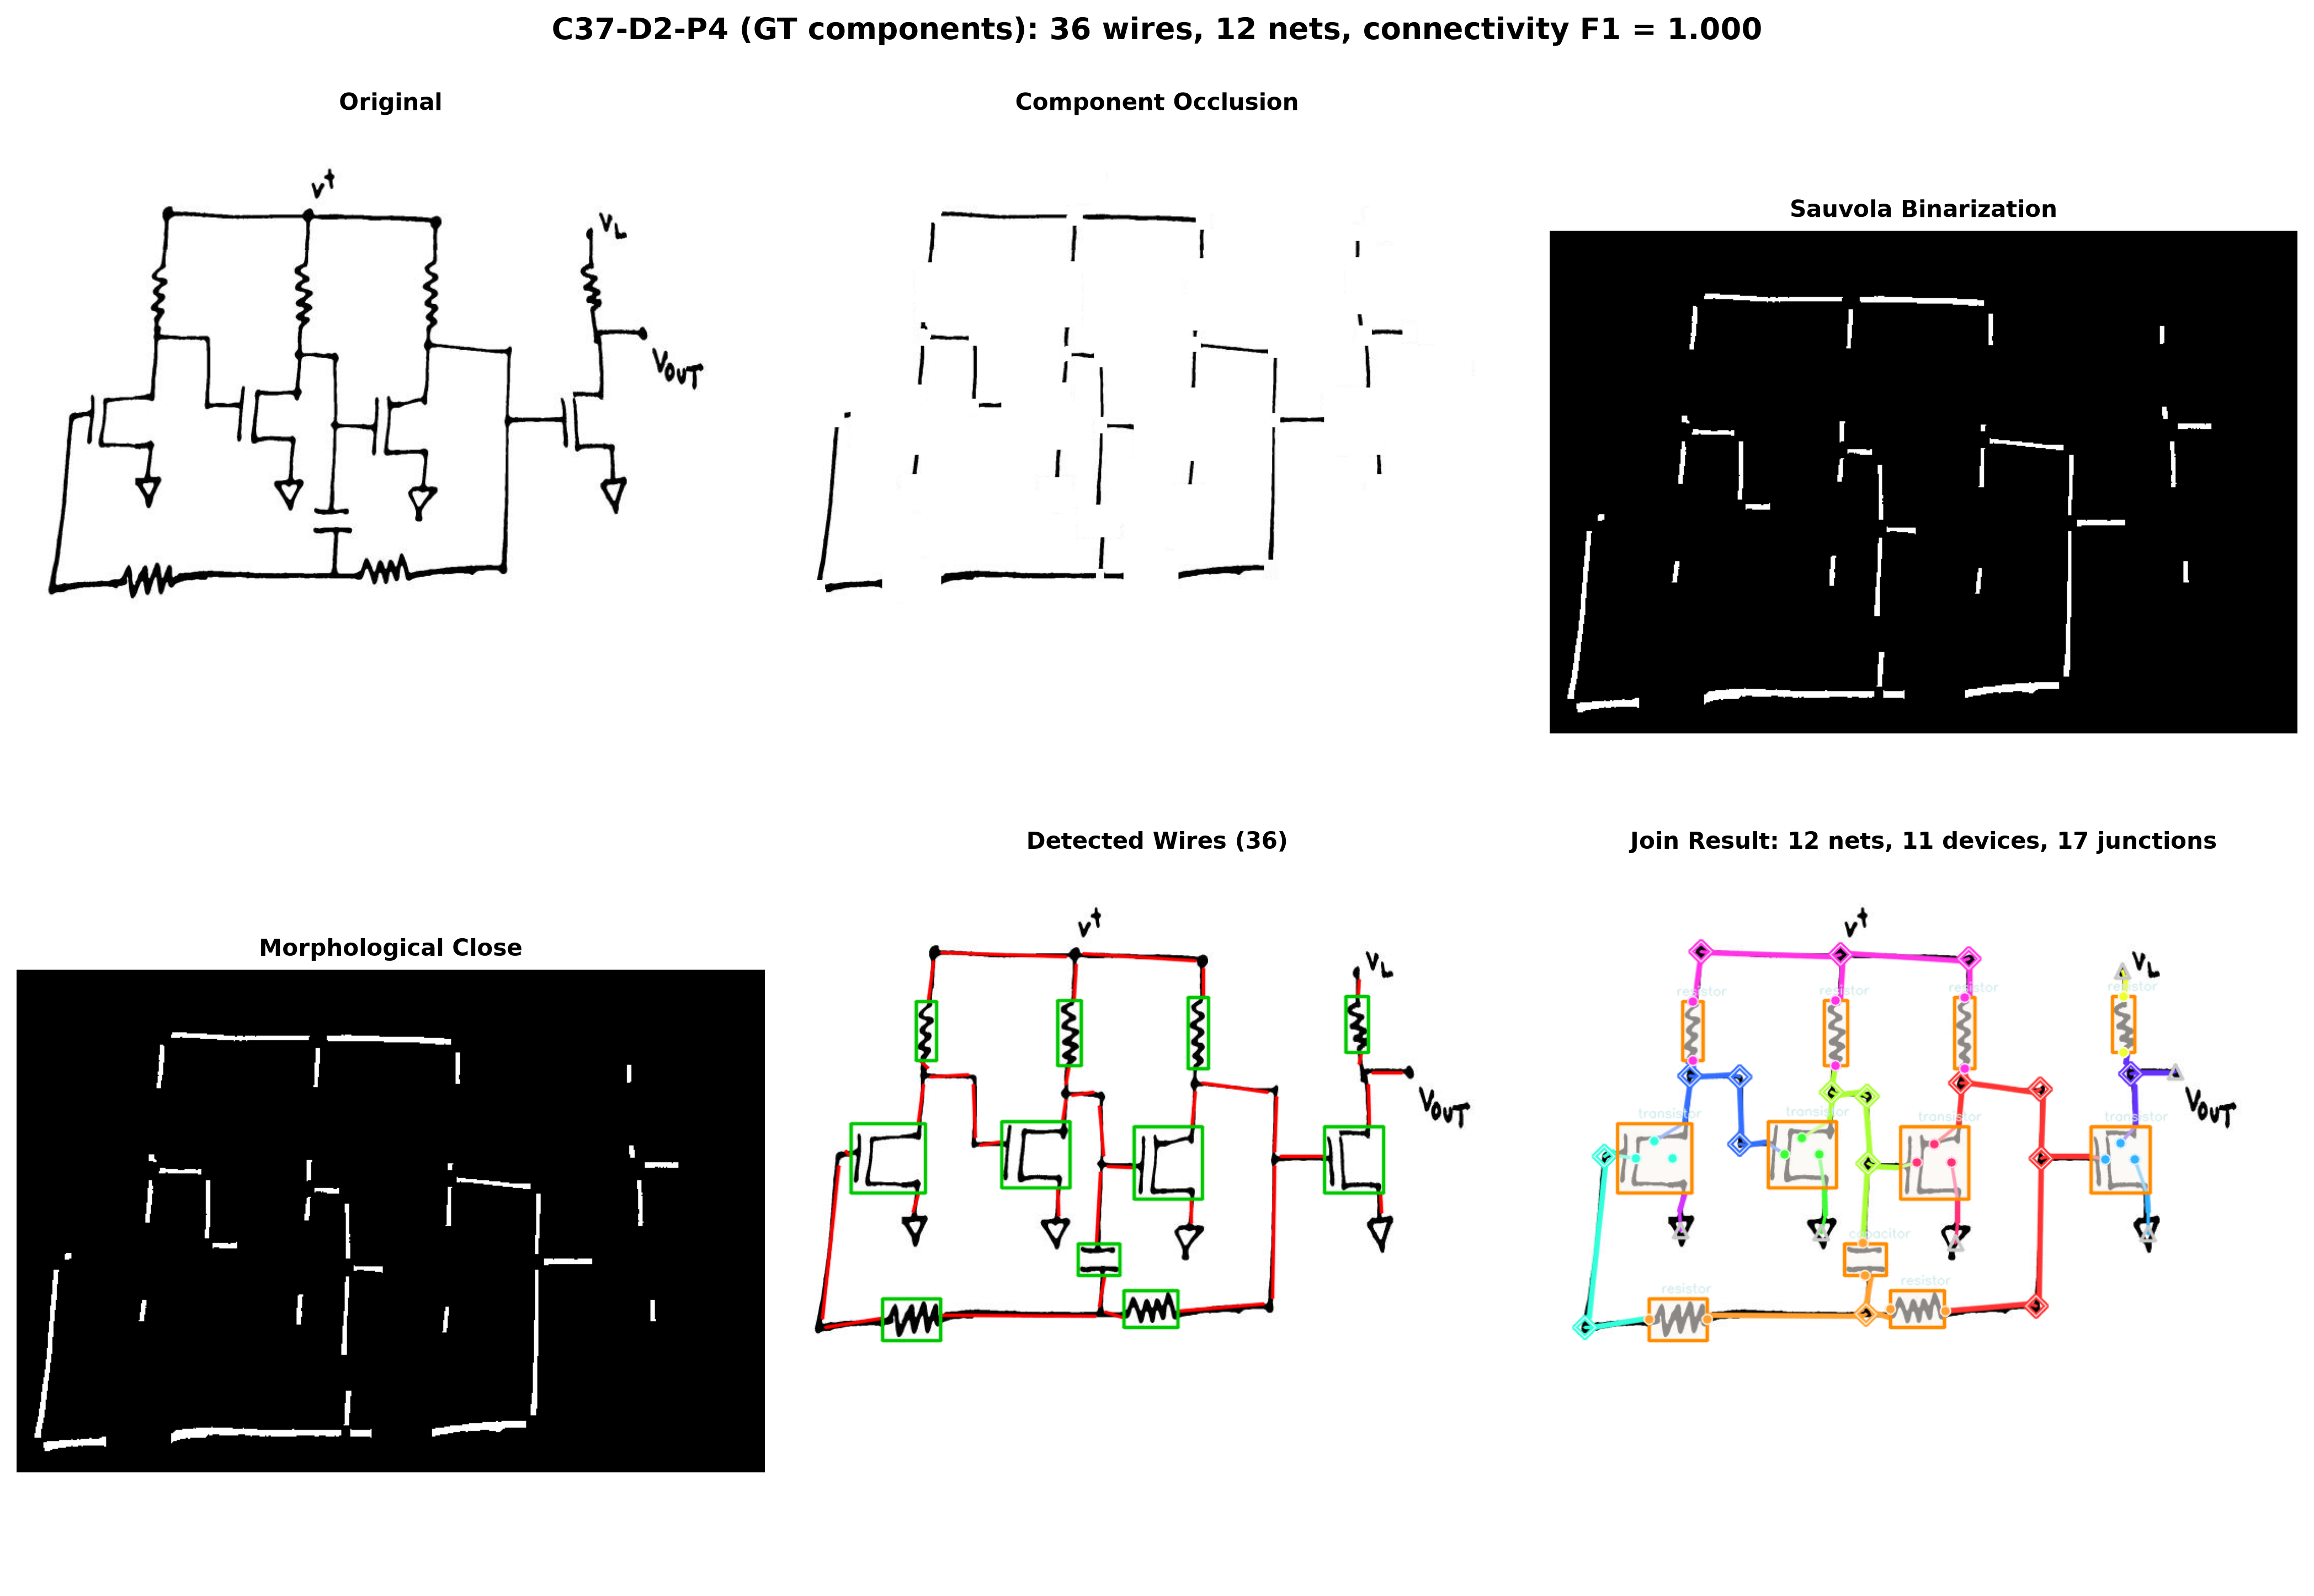
\includegraphics[width=0.48\textwidth]{figures/pipeline_examples/C37-D2-P4-jpg.png}
\hfill
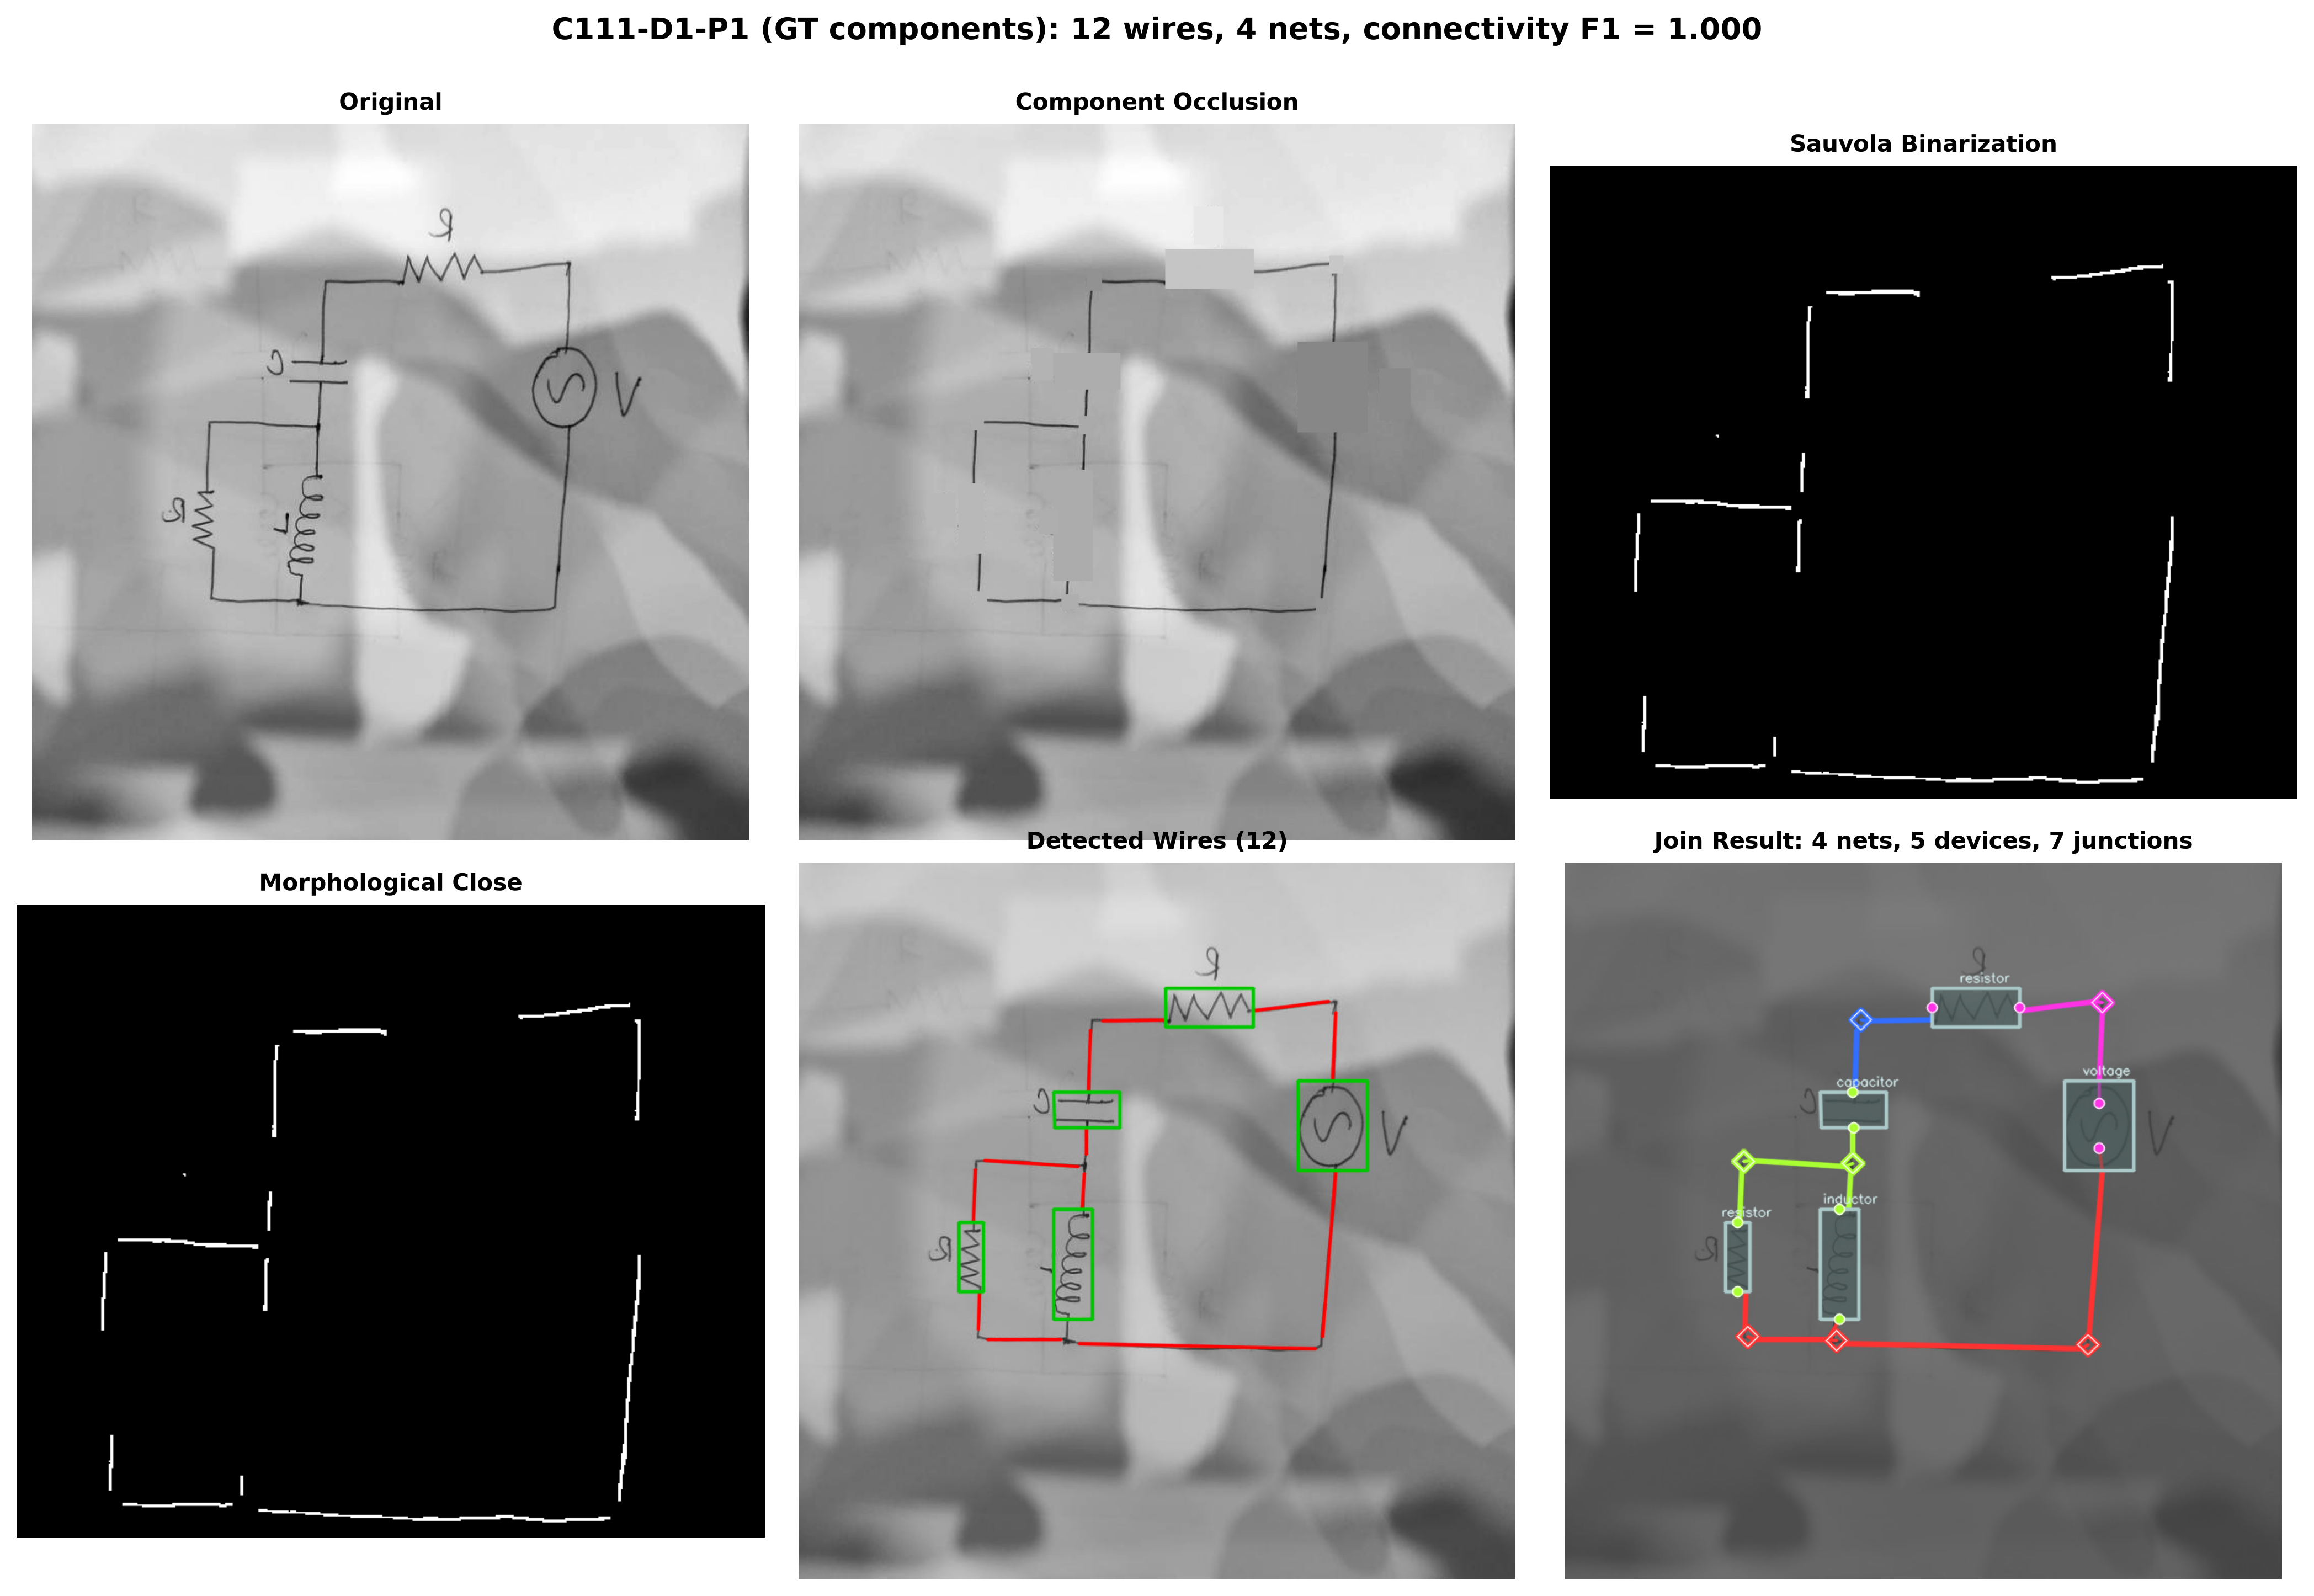
\includegraphics[width=0.48\textwidth]{figures/pipeline_examples/C111-D1-P1-jpg.png}
\caption{Pipeline stages on two real hand-drawn circuit images, joined with our scale-relative completion join (connectivity F1~=~1.000 on both). Left:~a four-transistor analog cell (35 wires, 7 nets); right:~an RLC loop photographed on a textured surface (11 wires, 4 nets). Each panel shows, in order: original scan, component occlusion, Sauvola binarization, morphological close, detected wires (red overlay), and the join result. In the join result every recovered net is a distinct colour drawn along its conductors; component bounding boxes are the ground-truth labels (as used throughout the net-level evaluation, isolating the join), filled dots are device pins, diamonds mark junctions, and triangles mark terminals and ground.}
\label{fig:pipeline_examples}
\end{figure*}

\section{Introduction}

Analog circuit schematics encode component types, values, and topological connections in a visual format designed for human interpretation. Recovering a structural netlist from a scan is a prerequisite for simulation, design verification, and large-scale circuit analysis, but a complete simulatable SPICE (Simulation Program with Integrated Circuit Emphasis) deck also requires component values and device models. This work addresses the structural connectivity stage only. The \emph{joining} problem determines which wire segments connect to which component pins and to each other. We study this stage with annotated component boxes; its relative contribution to autonomous reconstruction error is not established by that experiment.

The challenge is threefold. First, wire endpoints extracted from binarized images are inherently noisy: the same circuit drawn by different drafters produces endpoint positions that vary by 10--80 pixels. Second, components occupy bounding boxes that overlap with wire endpoints, creating ambiguity about whether an endpoint connects to a component's pin or merely passes nearby. Third, T-junctions, collinear fragments, and crossing wires create connectivity ambiguities for proximity-based rules, including the graph rules studied here.

A complementary approach is to prompt a vision-language model (VLM) for connectivity. Section~\ref{sec:vlm_results} reports an oracle-component-box diagnostic in which both methods receive the same annotated component boxes and the geometric method uses detected wires. The observed component-pair scores do not establish equivalence, comparative cost superiority or a global structural-validity guarantee. The diagnostic examines the methods under those stated input conditions.

We address these challenges with a deterministic structural-netlist pipeline whose proposed elements are: (1)~an \emph{occlusion-first wire extractor} that masks detected components before binarization and estimates per-segment endpoints, producing a line-segment-with-endpoints representation (rather than tracing nets directly into connected components, as prior systems do) that is what makes graph-based joining possible; (2)~an \emph{endpoint-graph join} model that constructs a graph over both wire endpoints and component pins, with five edge types capturing distinct connectivity patterns; and (3)~a \emph{degree-budget completion} algorithm that proposes recovery connections using bounded assignment and merge guards. We evaluate on the CGHD-1152 dataset~\cite{bayer2021cghd} with a synthetic error injection framework and a human-verified net-level benchmark. We evaluate topological recovery with illustrative SPICE export; component values and device models require external specification, and simulation equivalence on real scans is not validated. The output records inferred pin-to-node assignments, whereas the primary metric measures component-pair connectivity rather than exact pin topology.

\section{Related Work}

The end-to-end conversion of schematic images into machine-readable netlists has progressed rapidly. Kelly and Cole~\cite{kelly2024digitizing} presented a pattern-recognition workflow for digitizing circuit schematics with an 86.4\% success rate, combining optical character recognition (OCR) for component values with network-graph construction. SINA~\cite{sina2026}, the closest contemporary system, pairs a YOLOv11 detector with connected-component labeling (CCL) and OCR, and invokes a vision-language model (VLM) for reference-designator assignment, reporting 96.47\% netlist-generation accuracy, a 2.72$\times$ improvement over the prior state of the art. SINA confines the VLM to symbolic labeling and derives nets from CCL proximity rather than trusting the VLM with connectivity, an insight we share (Section~\ref{sec:vlm_connectivity}). Masala-CHAI~\cite{masalachai2024} (Auto-SPICE) uses large language models to produce SPICE netlists from analog schematics at scale. Most directly comparable to our setting, the concurrent work of Peker et al.~\cite{peker2026} (IEEE Access, 2026) builds a fully automated image-to-SPICE pipeline for printed and hand-drawn transistor-level circuits, pairing YOLOv8/11 detection with a \emph{contour-based} node-detection module (components are erased and nets are read from the contours of the residual wire pixels) and validates netlists by automated LTspice simulation against a reference. On their in-house seven-topology MOSFET dataset they report 93.33\% (printed) and 85.33\% (hand-drawn) whole-netlist success. Their node detection is an instance of the connected-component/contour recipe we evaluate as a baseline (Section~\ref{sec:real_eval}); because their dataset (transistor-level analog, authored in-house) and metric (LTspice node-voltage pass/fail) differ from ours (discrete components on CGHD-1152, component-pair F1), the headline numbers are not directly comparable. Our controlled comparison evaluates a CCL baseline on identical detected wires, rather than reproducing their complete system. Instance-segmentation approaches extract circuit graphs directly from pixels: Bayer et al.~\cite{instanceseg2023} segment components and wires for graph extraction over the CGHD lineage. For hand-drawn inputs, object-detection pipelines~\cite{handdrawn2021} and the recent JUHCCR-v1 database~\cite{juhccr2025} target component recognition on freehand sketches. Most of these pipelines build on general-purpose object detectors such as the YOLO family~\cite{redmon2016yolo,jocher2023yolo} and OCR engines such as Tesseract~\cite{smith2007tesseract}, with the ultimate goal of producing simulator-ready descriptions in formats such as SPICE~\cite{nagel1973spice}. These works address detection, recognition and connectivity under different datasets and metrics. Our contribution evaluates joining under specified component priors, without treating detection or recognition as solved. SPICE-level circuit modeling likewise underpins application deployment in neighboring hardware domains, including memristor-based neuromorphic circuits that realize brain-inspired learning in hardware~\cite{gao2026memristor} and memristive decision-making frameworks for autonomous navigation~\cite{gao2026memristive}.

Progress depends on annotated corpora. The CGHD hand-drawing dataset~\cite{bayer2021cghd} provides component- and wire-level annotations for handwritten schematics. In the analog/mixed-signal (AMS) domain, AMSnet~2.0~\cite{amsnet2025} contributes a large database built with AI-assisted segmentation for net detection, while AMSBench~\cite{amsbench2025} is a benchmark for evaluating multimodal LLM capabilities across AMS circuit tasks. Beyond circuits, DiagramNet~\cite{diagramnet2026} introduces an end-to-end framework and dataset for non-standard system-level diagrams, including an explicit connection-recognition task scored by F1. These benchmarks provide context for component recognition and connectivity evaluation. Our synthetic perturbation protocol isolates joining under authored errors; it does not measure the relative autonomous error contributions of those stages.

\label{sec:vlm_connectivity}
General-purpose VLMs and LLMs have been applied broadly to electronic design~\cite{llm4eda2024}, and to circuit understanding in particular. Kulkarni et al.~\cite{kulkarni2025enhancing} proposed Near Sight Correction using VLMs, reporting 87.4\% accuracy on circuit visual question answering (VQA) and 0.87 F1 on connection-matrix prediction. Connectivity-specific benchmarks report results that depend on the task, model and input conditions. On the DiagramNet connection task~\cite{diagramnet2026}, leading general models score very low F1 (GPT-5 at 0.029, Claude-Sonnet-4 at 0.265, and Gemini-2.5-Pro at 0.008), whereas a task-tuned 3B model reaches 0.735. AMSBench~\cite{amsbench2025} reports a similar gap for MLLMs on AMS connectivity. These task-specific results motivate a separately scoped connectivity diagnostic; they do not establish that geometry is superior to VLMs on our corpus. Our Claude-VLM experiment uses matched annotated component priors, as described in Section~\ref{sec:vlm_results}.

Classical wire extraction relies on edge detection, morphological operations, and the Hough transform~\cite{duda1972hough}, typically preceded by adaptive binarization such as Sauvola thresholding~\cite{sauvola2000} and connected-component labeling~\cite{he2017ccl}. Our legacy join baseline uses radius-based proximity: each wire endpoint grabs all component pins within a fixed threshold (typically 30px), connected via transitive union-find~\cite{tarjan1975union}. This can over-merge when multiple components fall within the threshold, assigning both pins of a two-terminal part (R, C, L, D) to the same net. SINA~\cite{sina2026} likewise derives nets from CCL proximity, which is similarly vulnerable to over-merge under detector noise. We instead model joining as a typed endpoint graph that incorporates component geometry and directional preference, and resolve residual ambiguity with a degree-budget completion: a bounded $b$-matching formulation~\cite{kuhn1955,schrijver2003combinatorial} that caps per-pin degree and thereby limits over-merge when endpoints are dropped or displaced. This differs from graph neural networks for netlist reverse engineering~\cite{alrahis2021gnn}, which learn representations over already-extracted gate-level graphs; our graph is a purely \emph{geometric} model whose edges encode spatial relationships between wire endpoints and component pins. A complementary recent direction replaces rule-based connectivity with a \emph{learned} model: Netlistify~\cite{netlistify2025} predicts terminal connectivity with a Transformer and reports a 12.4\% F1 gain over AMSnet on printed AMS schematics. Such models use task-specific connectivity training data. Transfer of the cited printed-schematic model to this hand-drawn benchmark is not established here; our geometric join requires no connectivity training. Open hand-drawn efforts such as CircuitNet~\cite{circuitnet} likewise rely on traditional image processing plus a classifier and a heuristic netlist generator.

\section{Method}

\subsection{Pipeline Overview}

Figure~\ref{fig:pipeline} summarizes the six-stage pipeline. The full pipeline proceeds through six stages: (1)~component detection via oriented bounding box (OBB) YOLO model; (2)~component occlusion (filling detected regions with local median color); (3)~Sauvola adaptive binarization; (4)~connected component labeling with morphological post-processing; (5)~wire endpoint extraction via principal component analysis (PCA) on endpoint regions; and (6)~wire joining via the endpoint-graph model with degree-budget completion. The output is a structural netlist mapping inferred component pins to electrical nodes. Component-pair evaluation does not certify those pin assignments or the exact net partition. SPICE export is illustrative: component values and device models require external specification, and simulation equivalence on real scans is not validated. Figure~\ref{fig:pipeline_examples} shows two representative circuits at each stage.

\subsection{Endpoint-Graph Join Model}

Given a set of wire segments $\mathcal{W} = \{w_1, \ldots, w_m\}$ with endpoints $\text{ep}(w_i) = (a_i, b_i)$ and component pins $\mathcal{P} = \{p_1, \ldots, p_n\}$, we construct an undirected graph $G = (V, E)$ where $V = \text{eps}(\mathcal{W}) \cup \mathcal{P}$.

\textbf{Edge type 1 (wire body):} For each wire $w_i$, add edge $(a_i,b_i)$ so both endpoints belong to the same net. The implementation accumulates connectivity with union-find; it does not solve a weighted graph optimization.

\textbf{Edge type 2 (endpoint--endpoint):} For endpoints $e_i,e_j$ on different wires with $\|e_i-e_j\|\leq\tau_{\text{join}}$, add an edge. This proximity rule can connect fragments, corners and junctions, but can also merge unrelated nearby wires.

\textbf{Edge type 3 (endpoint--pin):} Each endpoint is connected to at most one selected pin by this edge rule. First apply the component-first assignment described below. Only if no component is assigned, search pins within Euclidean distance $d\leq\tau_{\text{pin}}$ and select the pin with the smallest score. The score is $d$ unless directional preference is enabled and $d>10^{-6}$\,px; in that case it is $d[1-\alpha\max(0,\cos\theta)]$, with fixed $\alpha=0.35$ and $\theta$ measured from the outward wire direction to the endpoint-to-pin vector. Directional preference is enabled in the scale-relative base, but applies only to this fallback search. If an assigned component has no eligible pin, or the fallback finds none, no endpoint--pin edge is added. The score selects a fallback pin; it is not a weight optimized over the final graph.

\textbf{Edge type 4 (endpoint--wire-body):} For an endpoint $e$ and a different wire segment $w_j$, add an edge if the point-to-segment distance is at most $\tau_t$ and the normalized projection parameter lies in $[0.15,0.85]$. This rule represents T-junction candidates away from the segment ends.

\textbf{Edge type 5 (pin--wire-body):} For a component pin $p$ and wire segment $w_j$, add an edge if the point-to-segment distance is at most $\tau_t$ and the normalized projection parameter lies in $[0.05,0.95]$. This rule represents pin-to-rail candidates along a wire's body; geometric proximity alone does not certify an electrical connection.

The tolerances are manually configured scale-relative rules with fixed pixel clamps: $\tau_{\text{pin}}=\min(60,\max(24,0.62s))$, $\tau_{\text{join}}=\min(28,\max(11,0.30s))$, and $\tau_t=\min(20,\max(8,0.20s))$, in pixels. Here $s$ is the characteristic component-bounding-box diagonal scale; the implementation uses the middle sorted diagonal (the upper middle for an even count), falling back to a wire-length scale when component geometry is unavailable or degenerate. The multipliers and clamps are fixed, not learned. Because $s$ is a single scalar per image, intra-image size variance is not modeled: a schematic mixing a large IC with small discrete symbols shares one tolerance per rule. Extreme-size performance was not evaluated by controlled image rescaling.

\textbf{Component-first pin assignment:} For edge type 3, we use a two-step assignment. First, compute the distance from each endpoint to each component's oriented bounding box (OBB): 0 inside the rectangle, otherwise the minimum distance to its edges. If four OBB vertices are unavailable, use axis-aligned bounding-box (AABB) distance instead. Assign the endpoint to the nearest component whose distance is within $\max(\tau_{\text{pin}}, 0.5 \cdot \text{diagonal})$, where the diagonal is computed from that component's AABB. Second, within the assigned component, select the pin with the smallest Euclidean distance to the endpoint. Figure~\ref{fig:endpoint_graph} contrasts the legacy radius join with our endpoint-graph model.

\begin{figure*}[t]
\centering
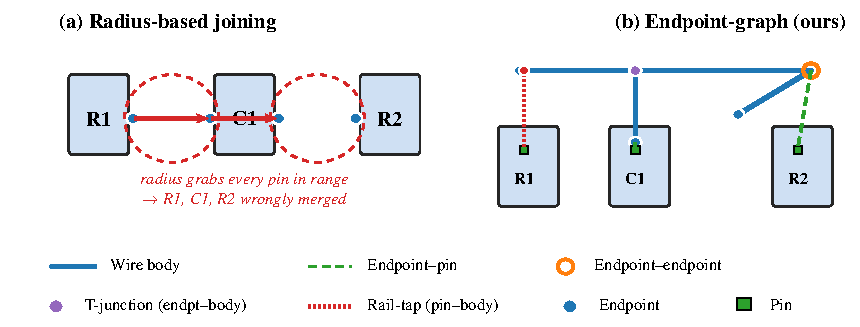
\includegraphics[width=\columnwidth]{figures/endpoint_graph.pdf}
\caption{Joining approaches compared. (a)~Radius-based join (legacy): each wire endpoint grabs all pins within a fixed threshold, causing over-merging. (b)~Our endpoint-graph model: typed edges and component-first pin assignment generate connectivity candidates, with directional scoring confined to the fallback pin search. Incorrect base merges remain possible.}
\label{fig:endpoint_graph}
\end{figure*}

Nets are computed as connected components of $G$, projected onto pins. The result is a netlist mapping each pin to a net identifier.

\subsection{Degree-Budget Completion}

The endpoint-graph join may leave a pin in a net containing only pins from its own component. Completion treats such pins as candidates for recovery, excluding inert types such as ground, supply markers, text, antenna, probes, junctions and terminals. This condition can reflect a missing connection, but does not establish that the detector dropped a wire.

Degree-budget completion retains the base net assignments and constructs candidates from each floating pin $p$ to pins $q$ on other components and different current nets. Candidate distance must not exceed $r=\rho\tau_c$, where $\tau_c=\min(60,\max(24,0.62s))$\,px and the deployed scale-relative completion uses $\rho=4$. Thus reach uses the clamped pin scale, not the raw component diagonal; completion retains this scale dependence when base tolerances are ablated. For each candidate, a wire witness is sought by pairing the endpoints of a detected segment with $p,q$ in either orientation. The witness cost is the smallest, over feasible segments and orientations, of the larger endpoint-to-pin distance, bounded by $r$. If no witness exists, the deployed relaxed-witness mode uses $\|p-q\|$ as the candidate cost.

When candidates exist, the implementation builds a rectangular assignment matrix with one row per floating pin. Each target pin supplies up to three distinct slot columns, limited by its candidate demand, and each row has a private dummy column with cost $1.5r$ for opting out. Unavailable assignments carry sentinel cost $10^6$. The Hungarian algorithm~\cite{kuhn1955} (\texttt{scipy.optimize.linear\_sum\_assignment}) assigns every row to exactly one column, with at most one row per column. This mandatory assignment with dummy options avoids the empty-solution ambiguity of a nonnegative-cost objective with only at-most-one constraints; target slots implement the bounded-capacity matching~\cite{schrijver2003combinatorial}.

Matches are then applied sequentially. Dummy or unavailable assignments add no edge. A proposed merge is also skipped if its endpoints are already in the same net or if their current nets share a component. This guard limits additional completion merges; it does not undo incorrect base unions or guarantee globally short-free output. Rejected matches are not reassigned, so the final guarded result is not claimed to minimize the assignment objective over all valid netlists.

Completion edges are ``wireless'': they represent inferred connections without corresponding wire segments, analogous to manual pin merges in schematic editors. Figure~\ref{fig:completion} illustrates the completion step.

\begin{figure*}[t]
\centering
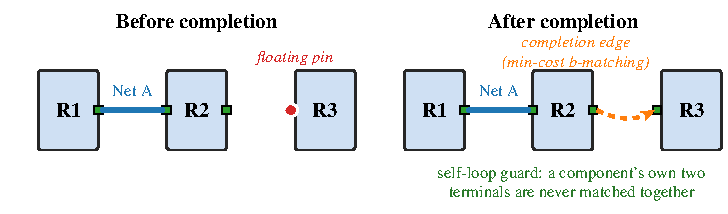
\includegraphics[width=\columnwidth]{figures/completion.pdf}
\caption{Degree-budget completion. Left: After base joining, some pins are ``floating'' (touching only their own component). Right: Completion reconnects floating pins via min-cost $b$-matching (orange dashed), with a guard rejecting additional merges between nets that already share a component; existing base shorts are not repaired.}
\label{fig:completion}
\end{figure*}

\section{Results}

\subsection{Synthetic Evaluation Framework}

We author 15 synthetic circuits spanning 3--6 components and 2--6 nets, including parallel resistors, series dividers, Wheatstone bridges, RC/RL circuits, diode loops, and a 6-component ring (cyclic and bridge topologies being the main stress cases for join robustness). Each circuit has a known ground-truth netlist and SPICE deck with a test voltage source.

We inject five categories of error at four severity levels (L1--L4) on top of the clean (L0) baseline. These are Gaussian endpoint jitter with standard deviation $\sigma$ (from 3\,px at L1 to 14\,px at L4), cut-short corruption in which each wire is shortened inward by a fixed length to model endpoints that stop short of the pin (from 4\,px at L1 to 22\,px at L4), full wire drops with probability $p_{\text{drop}}$ (up to 0.20 at L4), wrong-pin snaps with probability $p_{\text{wp}}$ (from 0.02 at L2 to 0.10 at L4), and anchor displacement, where with probability $p_{\text{disp}}$ one endpoint is moved by up to $a_{\max}$ pixels (from 30\,px at L1 to 80\,px at L4).

We report join F1 as the component-connectivity F1 score, measuring which unordered pairs of components share a net in the predicted versus ground-truth netlist. This metric discards terminal identity: even a perfect component-pair score does not certify pin assignment, the exact net partition, absence of shorts, or simulation equivalence. We report simulation accuracy as the percentage of random seeds for which every source current in the predicted SPICE netlist matches the clean oracle within 5\%.

\subsection{Wire Detection Benchmark}

We evaluate on 134 images from CGHD-1152 with ground-truth wire and component labels. Figure~\ref{fig:wire_benchmark} and Table~\ref{tab:wire_benchmark} summarize the top configurations across 36 tested variants.

\begin{figure}[t]
\centering
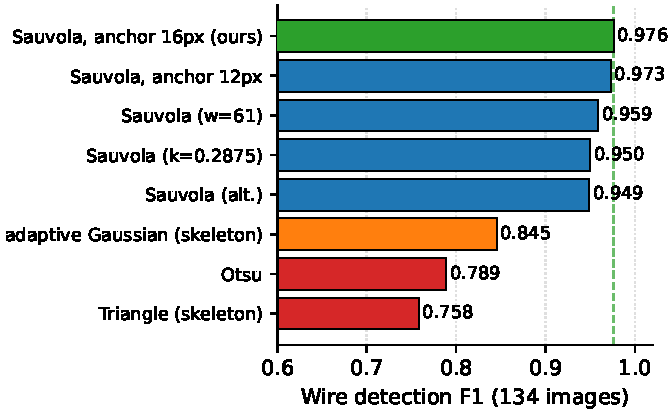
\includegraphics[width=\columnwidth]{figures/wire_benchmark.pdf}
\caption{Wire detection F1 across the tested thresholding methods and pipeline variants (134 images, annotated component boxes). The historical Sauvola configuration with a 16\,px anchor filter and overlap deduplication at $10^{\circ}$/18\,px achieves F1~=~0.976; this is distinct from the production $12^{\circ}$/8\,px deduplication setting. The adaptive Gaussian and Triangle bars use the stored skeleton-extraction configurations (F1~=~0.845 and 0.758, respectively).}
\label{fig:wire_benchmark}
\end{figure}

\begin{table}[htbp]
\caption{Wire detection performance on 134 images with annotated component boxes. The two Sauvola anchor-distance rows use historical $10^{\circ}$/18\,px overlap deduplication; they are not the production $12^{\circ}$/8\,px configuration.}
\label{tab:wire_benchmark}
\begin{center}
\begin{tabular}{lccc}
\toprule
\textbf{Configuration} & \textbf{F1} & \textbf{Prec} & \textbf{Rec} \\
\midrule
Sauvola + anchor 16\,px (ours) & \textbf{0.976} & 0.973 & 0.978 \\
Sauvola + anchor 12\,px & 0.973 & 0.974 & 0.972 \\
Sauvola ($w{=}61$) + anchor 12\,px & 0.959 & 0.944 & 0.974 \\
Sauvola ($k{=}0.2875$) + anchor 14\,px & 0.950 & 0.921 & 0.980 \\
Otsu threshold + CCL & 0.789 & 0.796 & 0.783 \\
\bottomrule
\end{tabular}
\end{center}
\end{table}

The historical 16\,px-anchor configuration achieves median F1 1.000, with 87\% of benchmark images scoring F1 at least 0.90. Its aggregate F1 is 0.9755 at $10^{\circ}$/18\,px overlap deduplication; the $12^{\circ}$/8\,px production configuration gives 0.9726 with the same 16\,px anchor distance. Among the tested alternatives, Otsu yields F1 0.789 and adaptive Gaussian 0.845. Occlusion is intended to remove component internals before wire extraction, but a full occlusion-removal ablation is not reported here; no quantified gain from that intervention is claimed.

\subsection{Join Strategy Comparison}

Table~\ref{tab:join_leaderboard} and Figure~\ref{fig:join_comparison} compare joining strategies on the synthetic evaluation framework (15 circuits $\times$ 8 seeds, mean F1 over error levels L1--L4).

\begin{table}[htbp]
\caption{Join Strategy Leaderboard (Synthetic Eval)}
\label{tab:join_leaderboard}
\begin{center}
\footnotesize
\setlength{\tabcolsep}{4pt}
\begin{tabular}{lccccc}
\toprule
\textbf{Strategy} & \textbf{L0} & \textbf{L1} & \textbf{L2} & \textbf{L3} & \textbf{L4} \\
\midrule
Scale-rel.\ graph + completion (ours) & 1.00 & 1.00 & 1.00 & \textbf{0.96} & \textbf{0.95} \\
Rescue graph + completion & 1.00 & 1.00 & 1.00 & 0.95 & 0.94 \\
Rescue graph (base) & 1.00 & 1.00 & 1.00 & 0.94 & 0.90 \\
Scale-rel.\ graph (base) & 1.00 & 1.00 & 1.00 & 0.94 & 0.85 \\
Radius union-find (legacy) & 1.00 & 0.97 & 0.90 & 0.56 & 0.36 \\
Nearest-pin + bbox anchor & 1.00 & 0.97 & 0.89 & 0.38 & 0.32 \\
\bottomrule
\end{tabular}
\end{center}
\end{table}

On the authored synthetic suite at L4, the scale-relative graph with completion scores F1 0.95, rescue graph with completion 0.94, rescue graph alone 0.90, scale-relative graph alone 0.85 and radius union-find 0.36 (Table~\ref{tab:join_leaderboard}). These results compare the reported configurations under the specified perturbations. They do not establish that completion repairs every dropped connection or prevents all shorts. The scale-relative completion configuration also has the highest component-pair score among the deterministic configurations reported on the real-image benchmark (Section~\ref{sec:real_eval}). For readability, two intermediate synthetic variants whose scores round to rows shown are omitted: nearest-pin without anchoring, and the scale-relative base with end-extension but no dead-end rescue.

\begin{figure*}[t]
\centering
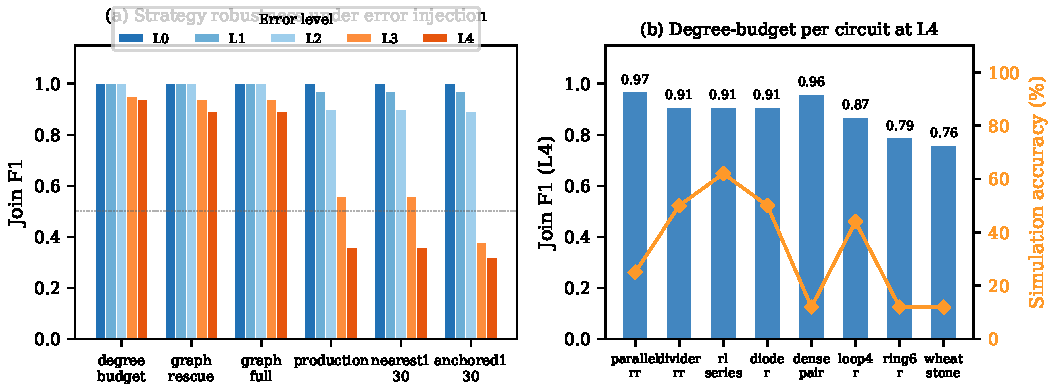
\includegraphics[width=\textwidth]{figures/join_comparison.pdf}
\caption{(a)~Join strategy robustness under error injection (15 circuits $\times$ 8 seeds): bars give mean connectivity F1 at each severity level (L0--L4, dark to light to red). The completion-based strategies (left) stay near 1.0, while the radius union-find and nearest-pin baselines (right) collapse at L3--L4. (b)~The scale-relative completion join per circuit at L4 (16 seeds): bars are connectivity F1, the orange line is simulation accuracy. High precision does not exclude false merges or certify pin correctness; the Wheatstone bridge has the lowest reported connectivity F1 and simulation accuracy (Table~\ref{tab:per_circuit}).}
\label{fig:join_comparison}
\end{figure*}

\subsection{Real-Image Net-Level Evaluation}
\label{sec:real_eval}

The synthetic results above measure robustness under an authored error model. For the real-image evaluation, we constructed a human-verified net-level benchmark of 31 CGHD-1152 images using a purpose-built verification tool. Thirty-four images were annotated; three were excluded before scoring (one pending human verification, two failing pre-registered physical-sanity checks), leaving the scored N=31. Net-level proposals were bootstrapped by a conservative endpoint-graph join over the dataset's annotated wires and then corrected by one human annotator. Human correction and evaluation on independently authored synthetic ground truth mitigate concern about method-dependent labels, but do not rule out residual bootstrap or annotator bias in the real benchmark. Both the geometric join and the VLM diagnostic receive annotated component boxes. Connectivity is scored as component-pair F1 restricted to the evaluated electrical-component subset, discarding terminal identities as in the synthetic connectivity metric.

Table~\ref{tab:real_join} reports the evaluated join configurations on the verified set, run on the pipeline's own detected wires. We report micro-averaged (pair-pooled) component-pair F1 as the primary metric, so that a dense 14-component board contributes in proportion to its connections rather than counting the same as a 3-component one; the macro (mean per-image) F1 is listed alongside for reference. The best configuration, the scale-relative completion join (degree-budget completion applied to a high-precision scale-relative endpoint-graph base), achieves micro-F1~=~0.890 (P~=~0.92, R~=~0.86; 95\% bootstrap CI [0.855, 0.924]), improving on the prior default that applies the same completion to the rescue base (0.829) and the radius union-find join (0.667) (Figure~\ref{fig:real_join_fig}). The scale-relative completion configuration omits the rescue base's 12\,px end-extension and dead-end rescue and has higher reported precision. This comparison does not isolate the causal contribution of those individual changes. A bounded within-benchmark reach sweep over $\rho\in[3,5]$, with $r=\rho\tau_c$, yields macro-F1 0.895--0.903. This is sensitivity evidence for the tested settings, not a controlled image-rescaling or mixed-size robustness experiment. Confidence intervals are wide at $N=31$ and the per-strategy intervals overlap, but the ranking is consistent and is corroborated on the independently authored synthetic suite (Table~\ref{tab:join_leaderboard}).

\begin{table}[htbp]
\caption{Leave-one-out ablation of endpoint-graph rules at the base-graph level and with completion, using annotated component boxes and detected wires on the 31-image benchmark. All full-pipeline rows have the same aggregate TP/FP/FN (418/37/66). Fixed-pixel base tolerances give micro-F1 0.820 versus 0.816 for the scale-relative base; completion retains its scale dependence. Aggregate ties do not establish identical recovered connections or a causal explanation for the ties.}
\label{tab:edge_ablation}
\centering
\begin{tabular}{lccccl}
\hline
Configuration & \multicolumn{2}{c}{Base graph only} & \multicolumn{3}{c}{Full pipeline} \\
\cline{2-3} \cline{4-6}
 & micro-F1 & TP/FP/FN & micro-F1 & P & R \\
\hline
Baseline (all edge types, scale-relative) & 0.816 & 352/27/132 & \textbf{0.890} & 0.919 & 0.864 \\
T-junctions disabled & 0.816 & 352/27/132 & 0.890 & 0.919 & 0.864 \\
Rail taps disabled & 0.816 & 352/27/132 & 0.890 & 0.919 & 0.864 \\
T-junctions + rail taps disabled & 0.816 & 352/27/132 & 0.890 & 0.919 & 0.864 \\
Directional preference disabled & 0.816 & 352/27/132 & 0.890 & 0.919 & 0.864 \\
Fixed-pixel base tolerances; completion unchanged & 0.820 & 356/28/128 & 0.890 & 0.919 & 0.864 \\
\hline
\end{tabular}
\end{table}

Table~\ref{tab:edge_ablation} reports bounded interventions on the base graph and the resulting pipeline with completion. Disabling T-junctions, rail taps or directional preference leaves the displayed base and full aggregate counts unchanged. Fixed-pixel base tolerances increase base micro-F1 from 0.816 to 0.820; the full-pipeline counts again tie at 418/37/66. Equal aggregate counts do not establish identical recovered connections, explain which mechanisms were active, or prove that completion masks differences. The baseline comparison shows an increase from base micro-F1 0.816 to 0.890 with completion, but these ablations do not establish that other mechanisms are generally unnecessary. Full occlusion removal and removal of scale dependence throughout completion were not tested. The ablation evidence therefore does not cover every proposed module or extreme-size input condition.

\begin{table}[htbp]
\caption{Join strategy and baseline comparison on human-verified net-level ground truth (31 real images, annotated component boxes; detected wires except for the stated perfect-wire reference). Primary metric is micro-averaged (pair-pooled) component-pair F1; macro (mean per-image) F1 is shown for reference.}
\label{tab:real_join}
\begin{center}
\footnotesize
\setlength{\tabcolsep}{4pt}
\begin{tabular}{lcccc}
\toprule
\textbf{Method} & \textbf{F1} & \textbf{Prec} & \textbf{Rec} & \textbf{F1$_{\text{macro}}$} \\
\midrule
\multicolumn{5}{l}{\emph{Deterministic joins (ours and ablations)}} \\
Scale-rel.\ graph + completion (ours) & \textbf{0.890} & 0.919 & 0.864 & \textbf{0.901} \\
Rescue graph + completion (prior) & 0.829 & 0.789 & 0.874 & 0.853 \\
Scale-rel.\ graph (base) & 0.816 & 0.929 & 0.727 & 0.838 \\
Rescue graph (base) & 0.787 & 0.811 & 0.764 & 0.813 \\
Radius union-find (legacy) & 0.667 & 0.698 & 0.638 & 0.674 \\
\midrule
\multicolumn{5}{l}{\emph{Classical deterministic baselines (identical detected wires)}} \\
Hough + proximity (best) & 0.805 & 0.750 & 0.868 & 0.847 \\
Connected-components (best) & 0.624 & 0.965 & 0.461 & 0.611 \\
\midrule
\multicolumn{5}{l}{\emph{Conditional VLM diagnostic / annotated-wire reference}} \\
VLM (Claude Opus~4.8) & 0.923 & 0.970 & 0.880 & 0.949 \\
Scale-rel.\ + completion, perfect wires & 0.890 & 0.913 & 0.868 & 0.916 \\
\bottomrule
\end{tabular}
\end{center}
\end{table}

\begin{figure}[t]
\centering
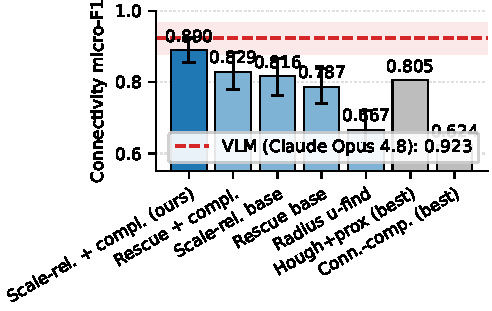
\includegraphics[width=\columnwidth]{figures/real_join_comparison.pdf}
\caption{Micro-averaged connectivity F1 on the 31-image human-verified net-level benchmark (component-pair metric). The scale-relative completion join has the highest score among the evaluated deterministic configurations and classical baselines on these detected wires. The dashed line marks the VLM diagnostic (Claude Opus 4.8). Both methods receive annotated component boxes; the VLM-minus-join difference is $+0.033$ (95\% bootstrap CI $[-0.009,+0.078]$). The interval does not establish equivalence, cost superiority or a global validity guarantee. Error bars are 95\% bootstrap CIs.}
\label{fig:real_join_fig}
\end{figure}

This real-image ranking resolves an open question from prior work on this pipeline: against bootstrapped pilot labels the degree-budget completion had \emph{not} consistently beaten its base join; against human-verified ground truth it clearly does (micro-F1 0.829 vs 0.787 for the rescue base alone), and the scale-relative variant is better still. The same ordering holds on the authored synthetic suite (Table~\ref{tab:join_leaderboard}), where the scale-relative completion join also ranks first, providing corroborating evidence on independently authored data without ruling out residual bias in the real benchmark labels.

Several image-to-netlist systems erase component regions and infer nets from the remaining wire pixels using connected components or contours, including SINA~\cite{sina2026} and Peker et al.~\cite{peker2026}. We evaluate a connected-component baseline on our detected wire segments to control the wire input. Its best tested configuration reaches component-pair micro-F1 0.624, versus 0.890 for the endpoint-graph join (Table~\ref{tab:real_join}). Hough line fitting~\cite{duda1972hough} followed by proximity linking reaches 0.805 at its best tested linking tolerance on the same detected wires. These are the best configurations in the reported sweeps, not upper bounds on all implementations of the classical methods. Their ordering is evidence for these configurations and this benchmark, not a direct performance comparison with the cited complete systems.

We additionally attempted to run five public image-to-netlist systems on the hand-drawn benchmark and encountered the following implementation, model-vocabulary and input-domain limitations. The classical printed-schematic interpreter of Kelly and Cole~\cite{kelly2024digitizing} installs and runs, but on hand-drawn scans it over-segments wires into spurious components and recovers almost no connectivity, a domain-transfer failure. Netlistify~\cite{netlistify2025} reproduces on its own printed AMS test data, which we ran end-to-end with the released model, but its active model lacks the diode, inductor, and IC classes our circuits contain and its connectivity model is trained on printed thin-line appearance, limiting its applicability to the device population in this benchmark. Masala-CHAI~\cite{masalachai2024} delegates connectivity to a proprietary LLM behind a paid API, equivalent in spirit to our VLM experiment in Section~\ref{sec:vlm_results}, rather than a deterministic algorithm. SINA's~\cite{sina2026} anonymized code archive was unextractable and CircuitNet~\cite{circuitnet} ships only Colab notebooks without released weights. These observations concern the versions and configurations examined; they do not establish that no prior system can recover hand-drawn connectivity. The CCL and Hough experiments above provide controlled comparisons on the same detected wires.

With annotated component boxes held fixed, replacing detected wires by the dataset's annotated wires changes component-pair micro-F1 from 0.8903 to 0.8898, while macro-F1 increases from 0.901 to 0.916 (Table~\ref{tab:real_join}). The micro scores round to the same displayed value, but are not identical. This comparison concerns wire input conditional on component annotations; it does not establish an autonomous detection bottleneck or exclude compensating changes in recovered connections.

\begin{figure}[t]
\centering
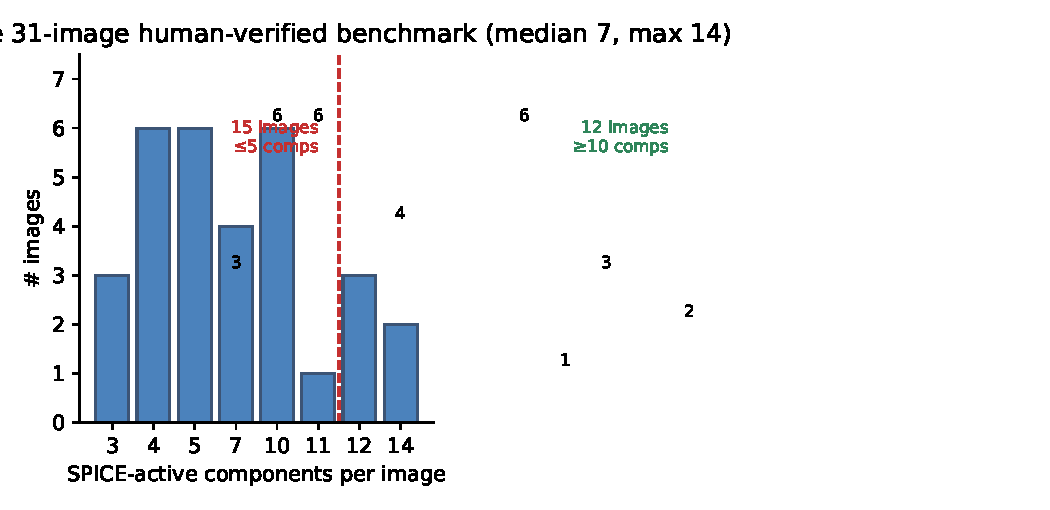
\includegraphics[width=0.82\textwidth]{figures/complexity_histogram.pdf}
\caption{Complexity of the 31-image human-verified benchmark, counting components in the evaluated electrical subset: 15 images have $\leq$5 and 12 have $\geq$10 (median 7, range 3--14). Component-count breadth does not validate dense buses or multilayer crossings; performance on these cases remains untested.}
\label{fig:complexity_hist}
\end{figure}

\subsection{Descriptive Per-Drafter Results}
Table~\ref{tab:per_drafter} reports the scale-relative completion join grouped by CGHD drafter. Drafter identities were recovered from the source tree for 16 of 31 images by direct filename match; the remaining 15 were inferred from the dataset's documented 12-circuits-per-drafter block structure. Four groups contain at least four images, with micro-F1 ranging from 0.854 to 0.987. These groups describe within-corpus variation, not evidence of unseen-drafter transfer. No held-out-drafter experiment was performed; the small, partly inferred groups do not support strong statistical separation.

\begin{table}[htbp]
\caption{Descriptive join micro-F1 (scale-relative completion) by CGHD drafter. Groups with at least four images; overall includes all benchmark images. Drafter identities include direct and inferred assignments.}
\label{tab:per_drafter}
\centering
\begin{tabular}{lcccc}
\hline
Drafter & $n$ images & micro-F1 & macro-F1 & TP/FP/FN \\
\hline
drafter\_1  & 7 & 0.933 & 0.907 & 56/6/2 \\
drafter\_2  & 5 & 0.854 & 0.874 & 85/14/15 \\
drafter\_10 & 5 & 0.987 & 0.995 & 37/1/0 \\
drafter\_12 & 4 & 0.913 & 0.938 & 21/0/4 \\
\hline
Overall    & 31 & 0.890 & 0.901 & 418/37/66 \\
\hline
\end{tabular}
\end{table}

\subsection{Per-Circuit Analysis}

Table~\ref{tab:per_circuit} shows the scale-relative completion join's performance across eight representative circuits from the 15-circuit synthetic corpus at L4 (extreme error injection, 16 seeds).

\begin{table}[htbp]
\caption{Scale-Relative Completion Join Performance per Circuit at L4 (16 seeds)}
\label{tab:per_circuit}
\begin{center}
\begin{tabular}{lrrrr}
\toprule
\textbf{Circuit} & \textbf{Comps} & \textbf{F1} & \textbf{Prec} & \textbf{Sim.\ acc.} \\
\midrule
Parallel R--R & 3 & 1.00 & 1.00 & 25\% \\
R--R divider & 3 & 0.99 & 1.00 & 69\% \\
RL series & 3 & 0.99 & 1.00 & 81\% \\
Diode--R loop & 3 & 0.99 & 1.00 & 69\% \\
Dual R loops & 4 & 0.93 & 0.90 & 12\% \\
4-component loop & 4 & 0.94 & 0.91 & 56\% \\
Wheatstone bridge & 6 & 0.82 & 0.85 & 6\% \\
6-component ring & 6 & 0.95 & 0.92 & 50\% \\
\bottomrule
\end{tabular}
\end{center}
\end{table}

Precision is at least 0.85 across the reported synthetic circuits at L4. This does not exclude false merges or establish that all errors are fragmentation. The Wheatstone bridge has the lowest reported F1 (0.82) and simulation accuracy of 6\%, illustrating that component-pair connectivity and the separately evaluated synthetic simulation criterion measure different properties.

\subsection{VLM Connectivity Experiment}
\label{sec:vlm_results}

We evaluate Claude Opus~4.8 as an oracle-component-box connectivity diagnostic. Both methods receive the same annotated component boxes; the geometric method uses detected wires. The VLM is given the scanned image with component boxes labelled by index and asked to return JSON sets of component terminals sharing an electrical node. Each image uses a separate model call without shared conversational context. We score the resulting unordered component pairs against the same human-verified benchmark. This is a conditional connectivity comparison, not an autonomous end-to-end comparison.

On the 31 real images, the VLM reaches micro-F1 0.923 (precision 0.970, recall 0.880; macro-F1 0.949), versus micro-F1 0.890 for the geometric join, and is exact under the component-pair metric on 21/31 images. The paired VLM-minus-join difference is $+0.033$, with 95\% bootstrap CI $[-0.009,+0.078]$. Inclusion of zero does not establish equivalence. These results do not establish comparative cost superiority or a global guarantee against incorrect merges for either method. Autonomous performance requires separately auditable evaluation; the conditional scores do not certify pin-level or simulation correctness.

\section{Discussion}
\label{sec:limitations}

The endpoint graph represents wire endpoints and component pins with separate rules for endpoint proximity, component assignment and mid-span contacts. Component-first assignment selects a nearby component by OBB distance and then a pin by Euclidean distance. These geometric choices provide inspectable connectivity candidates, but do not establish that a nearby wire is electrically connected or that a selected pin has the correct device-specific meaning.

Degree-budget completion proposes connections for pins left in single-component nets. Each floating-pin assignment selects at most one recovery target, and the shared-component guard can reject additional merges. Neither mechanism repairs shorts already present in the base graph. Wire-detection F1 does not measure an endpoint-drop rate or establish the causal contribution of missing endpoints to simulation failures.

The human-verified net-level evaluation, while novel for hand-drawn circuits, currently covers 31 images; the 95\% bootstrap confidence intervals on the per-strategy F1 are correspondingly wide ($\pm$0.03--0.05) and overlap between adjacent strategies, so while the top ranking is consistent and corroborated by the independently authored synthetic suite, broader annotation is needed to separate the closely ranked configurations. The net-level labels were bootstrapped by a conservative endpoint-graph join over perfect wires and then human-corrected; we mitigate the residual concern that this favors graph-based methods by validating on synthetic ground truth that is authored from scratch, where the same ranking holds. Annotation was performed by a single human annotator using a purpose-built verification tool, and no per-image timing log was retained, so a per-image annotation-cost figure cannot be reported. A proposed expansion protocol would stratify sampling by component count, drafter, crossing/bus structure and capture conditions, use independent annotation followed by adjudication, and record per-image effort and provenance logs. This is a proposed expansion protocol, not completed annotation. The evaluation draws from a single hand-drawn corpus (CGHD-1152); generalization across other drawing styles, capture conditions, and printed schematics remains to be validated.

Table~\ref{tab:capabilities} distinguishes the evaluated connectivity scope from generic pin guesses and illustrative export. Listing a device group does not establish separately detected model classes: the detector vocabulary merges multiple original classes. Pin construction depends on the component type supplied to the netlist stage; a template for a named complex device does not recover that identity from a merged detector label. Generic pin geometry is not evidence of validated device-specific pin relationships.

\begin{table*}[t]
\caption{Connectivity evaluation, generic pin construction, and illustrative export are distinct capabilities.}
\label{tab:capabilities}
\centering
\begin{tabular}{p{0.17\textwidth}p{0.24\textwidth}p{0.24\textwidth}p{0.24\textwidth}}
\toprule
Device group & Evaluated scope & Pin construction & Export limitation \\
\midrule
R/C/L/D/Q, voltage sources and ICs & Component-pair connectivity on the benchmark; no universal validation of pin templates & Geometric templates; endpoint clustering for eligible discrete/source types, generic layouts for ICs & Illustrative defaults/substitutions; values and device models require external specification. ICs are skipped because no export model is implemented. \\
Switches & Absent from the evaluated electrical subset; switch-specific connectivity unvalidated & Two pins from the shorter OBB-edge midpoints; long-axis AABB fallback & Fixed $0.001\,\Omega$ resistor if pins 0 and 1 map to distinct nodes; otherwise no switch line. No switch state or control model is recovered. \\
Transformers, thyristors, optocouplers and other complex devices & Device-specific connectivity unvalidated & Named transformer type receives a two-pin geometric guess; optocoupler template and unknown-type fallback also exist & These complex types have no implemented export model and are skipped; geometric guesses do not establish winding, control or isolation semantics. \\
Metric boundary (all evaluated groups) & Component pairs discard terminal identity & F1 does not certify pin assignment or the exact net partition & F1 does not certify absence of shorts or simulation equivalence. \\
\bottomrule
\end{tabular}
\end{table*}

Component detection has reported mAP@0.5 of 88.5\%, with crossover recall of 70.7\%. Geometric edge types 2, 4 and 5 do not consult crossover class labels when joining nearby wire fragments or mid-span contacts, creating a possible false-merge pathway. An audit using annotated component boxes found 13 crossover instances across eight benchmark images. In C242\_D1\_P1, suppressing two crossing-adjacent endpoint--endpoint edges changed component-pair TP/FP/FN from 27/4/0 to 19/0/8. Removing these edges also removes true connections; this is not a demonstrated mitigation gain. Detector-miss effects were not measured. This conditional joining intervention does not attribute the four false pairs to missed or misclassified detector outputs and is not a prevalence estimate. Crossover-aware suppression remains an unvalidated intervention, and the impact of crossover recognition errors on autonomous netlists remains unresolved.

The VLM comparison uses a single model (Claude Opus~4.8) on 31 images; evaluating additional models and prompting strategies is future work. The component detector was trained on CGHD-1152 after excluding drafter\_0, whose drawing style differed from the retained drafters; performance on that excluded style is not established here. The synthetic error model is an authored approximation rather than a calibrated fit to detector errors. Calibration to measured errors is future work.

\section{Conclusion}

We present structural circuit-netlist recovery using an occlusion-first wire extractor and endpoint-graph joining with degree-budget completion. On the 31-image within-corpus benchmark with annotated component boxes, component-pair micro-F1 is 0.8903; perfect-wire input gives 0.8898. These scores round alike but do not establish an autonomous detection bottleneck. The component-pair metric does not certify pin identities, exact net partitions, absence of shorts, or simulation equivalence. Synthetic L4 connectivity F1 is 0.95 versus 0.36 for the radius baseline. The VLM comparison is conditional on annotated component boxes and does not establish equivalence or cost superiority. Export remains illustrative: values and device models require external specification, and real-scan simulation equivalence is unvalidated. Broader styles, dense buses, and mixed-scale schematics require future evaluation.

% Funding moved to \tfootnote in the front matter (IEEE Access convention).

\section*{Acknowledgment}
The authors used Claude Opus 4.8 (Anthropic) to assist with grammar and language editing of the manuscript and as a programming assistant during development of the pipeline and evaluation code. This assistance is distinct from the VLM connectivity experiment in Section~\ref{sec:vlm_results}, where the same model is an evaluation subject. All methods, experiments, and conclusions are the authors' own, and the authors reviewed and take full responsibility for the entire content of this article.

\section*{Data and Code Availability}
The pipeline, evaluation scripts, synthetic-circuit generator, the 31-image
human-verified net-level ground truth (\texttt{ground\_truth/real\_nets\_verified.json}),
the net-level verification tool used to produce it, the join-strategy and
connected-component baseline benchmarks, and the Claude-VLM connectivity harness are
available at
\url{https://github.com/boscochanam/circuit-digitization}, including the per-image to CGHD drafter mapping used for the per-drafter analysis (Table~\ref{tab:per_drafter}). The component-detection model
is available at \url{https://huggingface.co/boscochanam/circuit-component-detector}, trained
on the CGHD-1152 dataset~\cite{bayer2021cghd}.

\begin{thebibliography}{00}
\bibitem{bayer2021cghd} F.~Thoma, J.~Bayer, Y.~Li, and A.~Dengel, ``A public ground-truth dataset for handwritten circuit diagram images,'' in \textit{Proc. Int. Conf. Document Analysis and Recognition (ICDAR)}, 2021, pp.~20--27. [Online]. Available: \url{https://doi.org/10.1007/978-3-030-86198-8_2}
\bibitem{kelly2024digitizing} C.~R.~Kelly and J.~M.~Cole, ``Digitizing images of electrical-circuit schematics,'' \textit{APL Mach. Learn.}, vol.~2, no.~1, p.~016109, 2024.
\bibitem{sina2026} S.~Aldowaish, Y.~Karumanchi, K.-C.~Chiang, S.~Noorzad, and M.~Fayazi, ``SINA: A circuit schematic image-to-netlist generator using artificial intelligence,'' in \textit{Proc. Design, Automation \& Test in Europe Conf. (DATE)}, 2026. [Online]. Available: \url{https://doi.org/10.23919/DATE69613.2026.11539285}
\bibitem{masalachai2024} J.~Bhandari, V.~Bhat, Y.~He, H.~Rahmani, S.~Garg, and R.~Karri, ``Masala-CHAI: A large-scale SPICE netlist dataset for analog circuits by harnessing AI,'' arXiv:2411.14299, 2024.
\bibitem{peker2026} \"{O}.~B.~Peker, E.~Toker, D.~\"{O}cal, T.~Dalyan, E.~Afacan, and Y.~D.~G\"{o}kdel, ``A fully automated SPICE-compatible netlist extraction from image using deep learning and image preprocessing techniques,'' \textit{IEEE Access}, vol.~14, pp.~19750--19765, 2026, doi: 10.1109/ACCESS.2026.3656316.
\bibitem{gao2026memristor} S.~Gao, F.~Shi, X.~Xu, J.~Chen, H.~H.-C.~Iu, et al., ``A memristor-based neural network circuit with classical conditioning and fear generalization,'' \textit{IEEE Trans. Consumer Electron.}, 2026, doi: 10.1109/TCE.2026.3663359.
\bibitem{gao2026memristive} S.~Gao, Y.~Song, Y.~Cao, H.~H.-C.~Iu, L.~Qin, Y.~Zhang, and J.~Mou, ``Biologically plausible memristive decision-making circuit for adaptive control in industrial autonomous navigation,'' \textit{IEEE Trans. Ind. Informat.}, vol.~22, pp.~4801--4812, 2026, doi: 10.1109/TII.2026.3668794.
\bibitem{instanceseg2023} J.~Bayer, A.~Roy, and A.~Dengel, ``Instance segmentation based graph extraction for handwritten circuit diagram images,'' in \textit{Proc. 12th Int. Conf. Pattern Recognition Applications and Methods (ICPRAM)}, 2023. [Online]. Available: \url{https://doi.org/10.5220/0011752600003411}
\bibitem{handdrawn2021} R.~R.~Reddy and M.~R.~Panicker, ``Hand-drawn electrical circuit recognition using object detection and node recognition,'' \textit{SN Comput. Sci.}, vol.~3, no.~3, p.~244, 2022. arXiv:2106.11559.
\bibitem{juhccr2025} A.~Roy, S.~Pani, S.~Malakar, and R.~Sarkar, ``JUHCCR-v1: A database for hand-drawn electrical and electronics circuit component recognition,'' \textit{Sci. Rep.}, vol.~15, art.~no.~22404, 2025, doi: 10.1038/s41598-025-22404-5.
\bibitem{redmon2016yolo} J.~Redmon, S.~Divvala, R.~Girshick, and A.~Farhadi, ``You only look once: Unified, real-time object detection,'' in \textit{Proc. IEEE Conf. Computer Vision and Pattern Recognition (CVPR)}, 2016, pp.~779--788.
\bibitem{jocher2023yolo} G.~Jocher, A.~Chaurasia, and J.~Qiu, ``Ultralytics YOLO,'' 2023. [Online]. Available: \url{https://github.com/ultralytics/ultralytics}
\bibitem{smith2007tesseract} R.~Smith, ``An overview of the Tesseract OCR engine,'' in \textit{Proc. 9th Int. Conf. Document Analysis and Recognition (ICDAR)}, 2007, pp.~629--633.
\bibitem{nagel1973spice} L.~W.~Nagel and D.~O.~Pederson, ``SPICE: Simulation program with integrated circuit emphasis,'' Electron. Res. Lab., Univ. California, Berkeley, Memo. ERL-M382, 1973.
\bibitem{amsnet2025} Y.~Shi, Z.~Tao, Y.~Gao, L.~Huang, H.~Wang, Z.~Yu, T.-J.~Lin, and L.~He, ``AMSnet 2.0: A large AMS database with AI segmentation for net detection,'' arXiv:2505.09155, 2025.
\bibitem{amsbench2025} Y.~Shi, Z.~Zhang, H.~Wang, Z.~Tao, Z.~Li, B.~Chen, Y.~Wang, Z.~Huang, X.~Liu, Q.~Chen, Z.~Yu, T.-J.~Lin, and L.~He, ``AMSbench: A comprehensive benchmark for evaluating MLLM capabilities in AMS circuits,'' arXiv:2505.24138, 2025.
\bibitem{diagramnet2026} J.~Lou, R.~Xu, J.~Li, J.~Pi, R.~Tao, W.~Fan, X.~Tan, G.~Luo, and Y.~Lin, ``DiagramNet: An end-to-end recognition framework and dataset for non-standard system-level diagrams,'' arXiv:2605.01338, 2026.
\bibitem{llm4eda2024} R.~Zhong, X.~Du, S.~Kai, Z.~Tang, S.~Xu, H.-L.~Zhen, J.~Hao, Q.~Xu, M.~Yuan, and J.~Yan, ``LLM4EDA: Emerging progress in large language models for electronic design automation,'' arXiv:2401.12224, 2024.
\bibitem{kulkarni2025enhancing} S.~Kulkarni \textit{et~al.}, ``Enhancing circuit diagram understanding via near sight correction using VLMs,'' in \textit{Proc. ICCV Workshops}, 2025.
\bibitem{duda1972hough} R.~O.~Duda and P.~E.~Hart, ``Use of the Hough transformation to detect lines and curves in pictures,'' \textit{Commun. ACM}, vol.~15, no.~1, pp.~11--15, 1972.
\bibitem{sauvola2000} J.~Sauvola and M.~Pietik\"{a}inen, ``Adaptive document image binarization,'' \textit{Pattern Recognit.}, vol.~33, no.~2, pp.~225--236, 2000.
\bibitem{he2017ccl} L.~He, X.~Ren, Q.~Gao, X.~Zhao, B.~Yao, and Y.~Chao, ``The connected-component labeling problem: A review of state-of-the-art algorithms,'' \textit{Pattern Recognit.}, vol.~70, pp.~25--43, 2017.
\bibitem{tarjan1975union} R.~E.~Tarjan, ``Efficiency of a good but not linear set union algorithm,'' \textit{J. ACM}, vol.~22, no.~2, pp.~215--225, 1975.
\bibitem{kuhn1955} H.~W.~Kuhn, ``The Hungarian method for the assignment problem,'' \textit{Naval Res. Logist. Quart.}, vol.~2, no.~1--2, pp.~83--97, 1955.
\bibitem{schrijver2003combinatorial} A.~Schrijver, \textit{Combinatorial Optimization: Polyhedra and Efficiency}. Berlin, Germany: Springer, 2003.
\bibitem{alrahis2021gnn} L.~Alrahis, A.~Sengupta, J.~Knechtel, S.~S.~Gharibeh, O.~S.~Unsal, M.~E.~Acar, and H.~Najjar, ``GNN-RE: Graph neural networks for reverse engineering of gate-level netlists,'' in \textit{Proc. IEEE/ACM Int. Conf. Computer-Aided Design (ICCAD)}, 2021, pp.~1--9.
\bibitem{netlistify2025} C.-Y.~Huang, H.-I.~Chen, H.-W.~Ho, P.-H.~Kang, M.~P.-H.~Lin, W.-H.~Liu, and H.~Ren, ``Netlistify: Transforming circuit schematics into netlists with deep learning,'' in \textit{Proc. ACM/IEEE Symp. Machine Learning for CAD (MLCAD)}, 2025.
\bibitem{circuitnet} ``CircuitNet: A hand-drawn schematic sketch recognizer and converter,'' GitHub repository (user aaanthonyyy), 2024. [Online]. Available: \url{https://github.com/aaanthonyyy/CircuitNet}
\end{thebibliography}

% ---- Author biographies (IEEE Access requires one for EVERY author) ----
% The class opens each bio with "\vskip \@IEEEBIOskipN plus 1fil", so leftover
% column space stretches into large gaps between bios. Cap that stretch and
% let spare space fall to the column bottom instead.
\makeatletter
% The env takes an optional arg, so its body lives in the internal
% macro \csname\string\IEEEbiography\endcsname, not \IEEEbiography.
\expandafter\patchcmd\csname\string\IEEEbiography\endcsname%
  {\vskip \@IEEEBIOskipN plus 1fil minus 0\baselineskip}%
  {\vskip \@IEEEBIOskipN plus 0.5\baselineskip minus 0\baselineskip}%
  {}{\typeout{WARNING: IEEEbiography spacing patch did not apply}}
\makeatother
\raggedbottom
\begin{IEEEbiography}[{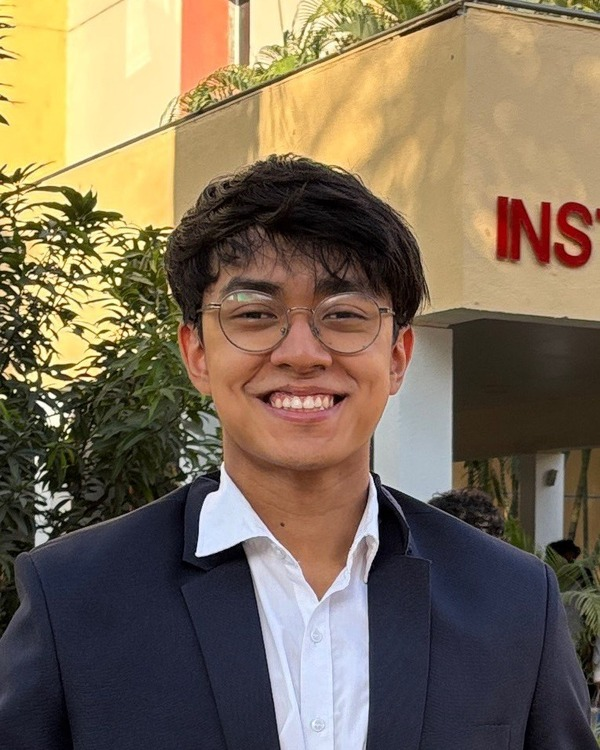
\includegraphics[width=1in,height=1.25in,clip,keepaspectratio]{figures/authors/chanam.jpg}}]{Bosco Chanam}
received the B.Tech.\ degree in Computer Science and Engineering from the Symbiosis Institute of Technology (SIT), Pune, India. He is currently an AI/ML Engineer at the AI Incubation Centre at Bharat Forge (Kalyani Group), Pune, India. His professional and research interests include computer vision, edge AI optimization, and robotics. Mr.~Chanam has co-authored research in natural language processing benchmarking, published in the \textit{International Journal of Fuzzy Logic and Intelligent Systems}.
\end{IEEEbiography}

\begin{IEEEbiography}[{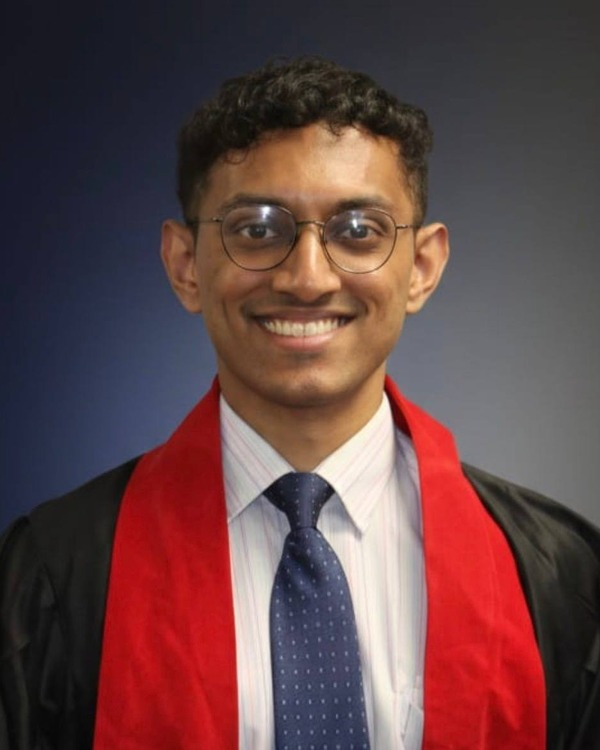
\includegraphics[width=1in,height=1.25in,clip,keepaspectratio]{figures/authors/dcosta.jpg}}]{Chris Dcosta}
received the B.Tech.\ degree in Computer Science and Engineering with Honors in Artificial Intelligence and Machine Learning from the Symbiosis Institute of Technology (SIT), Pune, India. His research interests include computer vision, machine learning, natural language processing, and deep learning.
\end{IEEEbiography}

\begin{IEEEbiography}[{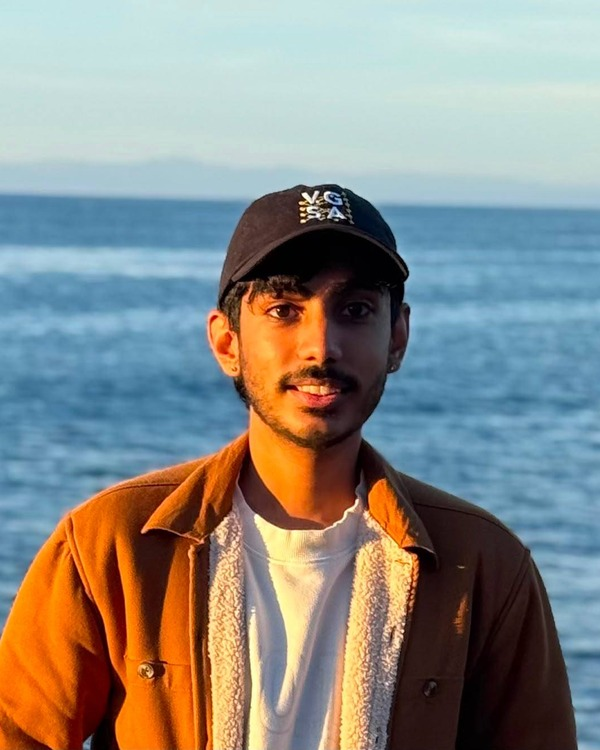
\includegraphics[width=1in,height=1.25in,clip,keepaspectratio]{figures/authors/talupuri.jpg}}]{Pranavesh Kumar Talupuri}
is with the Department of Computer Science, University of Southern California, Los Angeles, CA, USA. His research interests include machine learning, deep learning, and computer vision.
\end{IEEEbiography}

\begin{IEEEbiography}[{
\includegraphics[width=1in,height=1.25in,clip,keepaspectratio]{figures/authors/chiwhane.jpg}}]{Shwetambari Chiwhane}
holds a B.E. in Computer Science and Engineering from Sant Gadge
Baba Amravati University, Amravati, India, and an M.Tech. in Computer Science and Engineering
from Dr. Babasaheb Technological University, Lonere, India. She earned her PhD in Computer
Engineering specializing from Bharath Institute of Higher Education and Research, Chennai,
India. Presently, she serves as an Assistant Professor in the Department of Computer Science and
Engineering at Symbiosis Institute of Technology, Symbiosis International (Deemed University),
Pune, India, gathering over two decades of teaching and research expertise. She is life member of
ISTE.

Her contributions extend beyond academia; she has contributed as a reviewer for various
international conferences. Dr. Shwetambari’s research expertise is evident with her receiving many
publications. She has authored over 35 research articles in various international and national
conferences and journals. Her professional engagements include roles such as NAAC, NBA,
among others.

Recognized as a PhD guide in Symbiosis International (Deemed University), Presently she is
guiding 4 research scholar and she has guided more than 100 undergraduate students for their
research endeavors. Her current research interests revolve around Image Processing, Computer
Vision, Artificial Intelligence and Machine Learning.
\end{IEEEbiography}

\begin{IEEEbiography}[{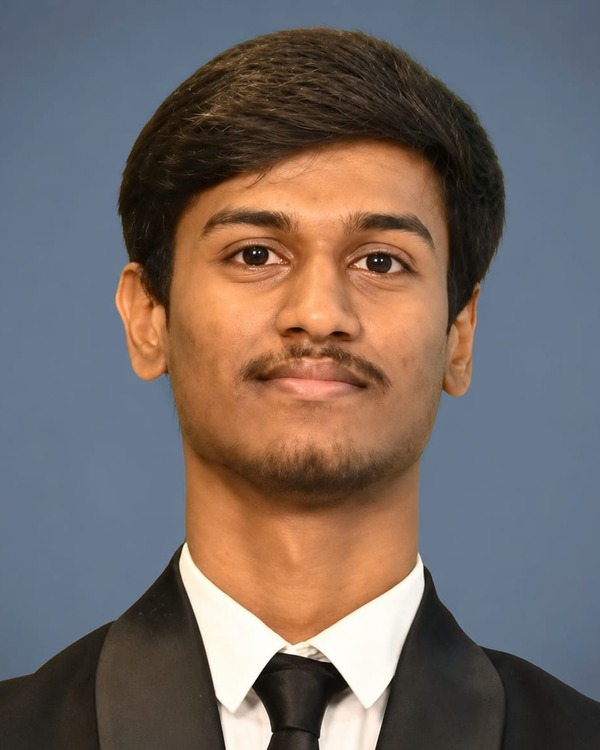
\includegraphics[width=1in,height=1.25in,clip,keepaspectratio]{figures/authors/singh.jpg}}]{Ashay Kumar Singh}
received the B.Tech.\ degree in Computer Science and Engineering from the Symbiosis Institute of Technology (SIT), Pune, India. His research interests lie in machine learning, computer vision, Retrieval-Augmented Generation (RAG), optical character recognition (OCR), and multimodal AI.
\end{IEEEbiography}

\begin{IEEEbiography}[{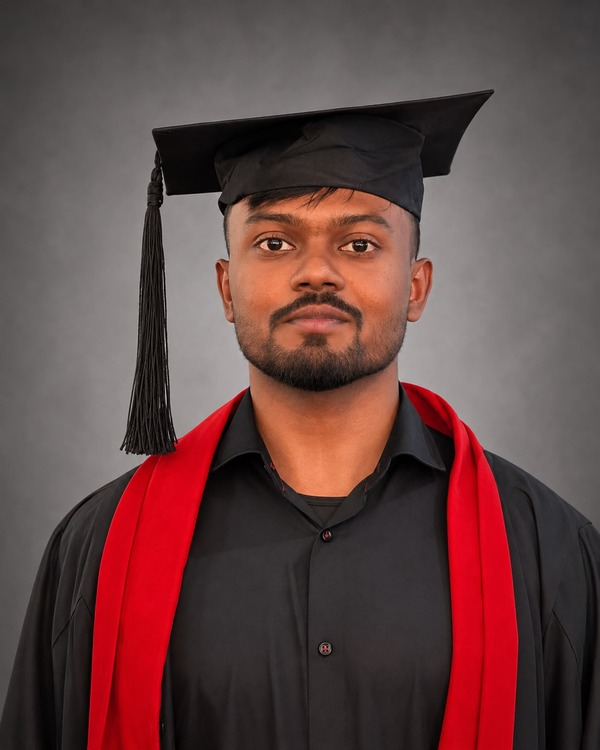
\includegraphics[width=1in,height=1.25in,clip,keepaspectratio]{figures/authors/das.jpg}}]{Arghadeep Das}
received the B.Tech.\ degree in Computer Science and Engineering from the Symbiosis Institute of Technology (SIT), Pune, India. His research interests include reinforcement learning, world models, computer vision, 3D rendering, agentic AI, embodied AI, robotics, and machine learning.
\end{IEEEbiography}

\EOD

\end{document}
